\documentclass[aspectratio=169]{beamer}
\usetheme{Madrid}
\usecolortheme{whale}

\usepackage{graphicx}
\usepackage{listings}
\usepackage{xcolor}
\usepackage{tikz}
\usetikzlibrary{shapes,arrows,positioning,calc}
\usepackage{booktabs}
\usepackage{adjustbox}

% Code listing style - escape special chars
\lstset{
    basicstyle=\ttfamily\tiny,
    keywordstyle=\color{blue},
    commentstyle=\color{gray},
    stringstyle=\color{orange},
    breaklines=true,
    frame=single,
    backgroundcolor=\color{gray!10},
    escapeinside={(*@}{@*)},
    literate={\_}{\_}1
}

\title{Hotel Recommendation Chatbot}
\subtitle{J.A.R.V.I.S.}
\author{
    \textbf{Team 42}\\[0.3cm]
    Omar Fouad \quad Jana Elewainy \quad Yara Tantawy \quad Ziad Elgendy
}
\date{\today}

\begin{document}

%==============================================================================
\begin{frame}
\titlepage
\end{frame}

%==============================================================================
% SECTION 1: HIGH-LEVEL SYSTEM ARCHITECTURE
%==============================================================================
\section{System Architecture}

\begin{frame}{System Architecture Overview}
\begin{center}
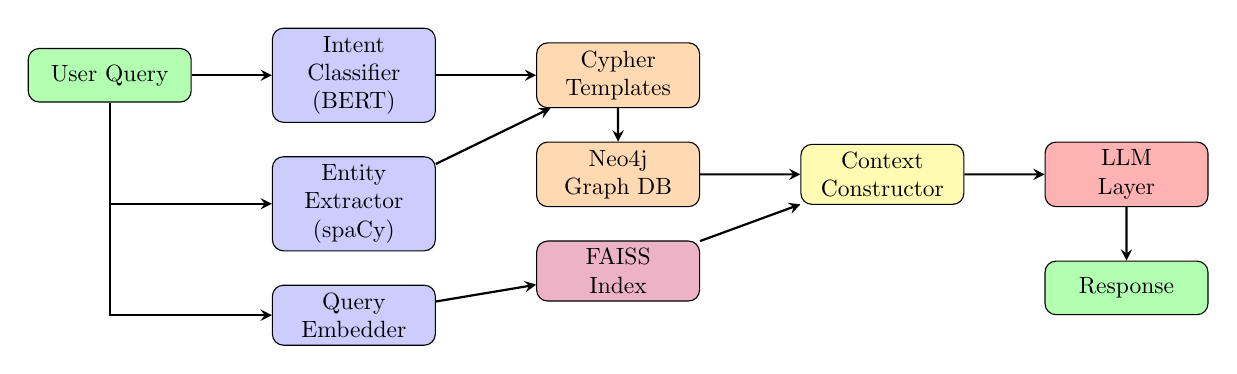
\begin{tikzpicture}[node distance=1.2cm, scale=0.85, transform shape,
    block/.style={rectangle, draw, fill=blue!20, text width=2.2cm, text centered, minimum height=0.8cm, rounded corners},
    arrow/.style={->, >=stealth, thick}]

    % Input
    \node[block, fill=green!30] (input) {User Query};

    % Preprocessing
    \node[block, right=of input] (intent) {Intent\\Classifier\\(BERT)};
    \node[block, below=0.5cm of intent] (entity) {Entity\\Extractor\\(spaCy)};
    \node[block, below=0.5cm of entity] (embed) {Query\\Embedder};

    % Retrieval
    \node[block, right=1.5cm of intent, fill=orange!30] (cypher) {Cypher\\Templates};
    \node[block, below=0.5cm of cypher, fill=orange!30] (neo4j) {Neo4j\\Graph DB};
    \node[block, below=0.5cm of neo4j, fill=purple!30] (faiss) {FAISS\\Index};

    % Context
    \node[block, right=1.5cm of neo4j, fill=yellow!30] (context) {Context\\Constructor};

    % LLM
    \node[block, right=of context, fill=red!30] (llm) {LLM\\Layer};

    % Output - below LLM instead of to the right
    \node[block, below=0.8cm of llm, fill=green!30] (output) {Response};

    % Arrows
    \draw[arrow] (input) -- (intent);
    \draw[arrow] (input) |- (entity);
    \draw[arrow] (input) |- (embed);
    \draw[arrow] (intent) -- (cypher);
    \draw[arrow] (entity) -- (cypher);
    \draw[arrow] (cypher) -- (neo4j);
    \draw[arrow] (embed) -- (faiss);
    \draw[arrow] (neo4j) -- (context);
    \draw[arrow] (faiss) -- (context);
    \draw[arrow] (context) -- (llm);
    \draw[arrow] (llm) -- (output);

\end{tikzpicture}
\end{center}

\vspace{0.3cm}
\textbf{Task:} Hotel Recommender: J.A.R.V.I.S.

\end{frame}

%==============================================================================
% SECTION 2: INPUT PREPROCESSING
%==============================================================================
\section{Input Preprocessing}

\begin{frame}{Intent Classification - Fine Tuning a BERT Model}
\begin{columns}
\begin{column}{0.5\textwidth}
\textbf{Model:} \texttt{bert-base-uncased}

\textbf{Dataset:} Custom labeled dataset (200 samples)
% \textbf{Training Config:}
% \begin{itemize}
%     \item Learning rate: 5e-5
%     \item Batch size: 16
%     \item Epochs: 15
%     \item Train/Test split: 85/15
% \end{itemize}

\vspace{0.3cm}
\textbf{10 Intent Classes:}
\begin{enumerate}
    \scriptsize
    \item hotel\_recommendation
    \item hotel\_search
    \item hotel\_info
    \item review\_query
    \item comparison
    \item traveller\_preference
    \item location\_query
    \item visa\_query
    \item rating\_filter
    \item general\_question
\end{enumerate}
\end{column}

\begin{column}{0.5\textwidth}
\textbf{Classification Examples:}

\vspace{0.2cm}
\scriptsize
\begin{tabular}{|p{3.2cm}|l|}
\hline
\textbf{Query} & \textbf{Intent} \\
\hline
``Recommend hotel in Tokyo'' & hotel\_rec (0.97) \\
\hline
``Do I need visa from India?'' & visa\_query (0.89) \\
\hline
``Compare Azure and Marina'' & comparison (0.94) \\
\hline
``Best for business travelers'' & traveller\_pref (0.91) \\
\hline
``Hotels with rating above 9'' & rating\_filter (0.88) \\
\hline
\end{tabular}
\end{column}
\end{columns}
\end{frame}

%------------------------------------------------------------------------------
\begin{frame}{Entity Extraction}
\begin{columns}
\begin{column}{0.4\textwidth}
\textbf{Approach:} spaCy NER + keyword lookups

\vspace{0.2cm}
\textbf{Entity Types Extracted:}
\begin{itemize}
    \scriptsize
    \item \textbf{Hotels} - FAC, ORG labels + lookup
    \item \textbf{Cities/Countries} - GPE label
    \item \textbf{Traveller Types} - Keyword lookup
    \item \textbf{Demographics} - Lookup + DATE
    \item \textbf{Ratings} - Numeric extraction
\end{itemize}

\vspace{0.2cm}
\textbf{Keyword Mappings:}
\begin{itemize}
    \scriptsize
    \item solo, alone $\rightarrow$ ``Solo''
    \item business $\rightarrow$ ``Business''
    \item cleanliness $\rightarrow$ cleanliness\_base
    \item senior $\rightarrow$ age ``55+''
\end{itemize}
\end{column}

\begin{column}{0.6\textwidth}
\textbf{Extraction Examples:}
\scriptsize

\vspace{0.1cm}
\texttt{``Best hotels for solo female in Paris''}
\begin{itemize}
    \scriptsize
    \item cities: [``Paris''], traveller\_types: [``Solo''], demographics: [``Female'']
\end{itemize}

\vspace{0.1cm}
\texttt{``Hotels with cleanliness above 9''}
\begin{itemize}
    \scriptsize
    \item cleanliness\_base: 9.0
\end{itemize}

\vspace{0.1cm}
\texttt{``Compare Azure Tower and Marina Bay''}
\begin{itemize}
    \scriptsize
    \item hotels: [``The Azure Tower'', ``Marina Bay'']
\end{itemize}

\vspace{0.1cm}
\texttt{``Hotels recommended for seniors''}
\begin{itemize}
    \scriptsize
    \item demographics: [``55+'']
\end{itemize}
\end{column}
\end{columns}
\end{frame}

%------------------------------------------------------------------------------
\begin{frame}{Input Embedding}
\begin{columns}
\begin{column}{0.5\textwidth}
\textbf{Query-to-Embedding Flow:}
\vspace{0.2cm}

\begin{center}
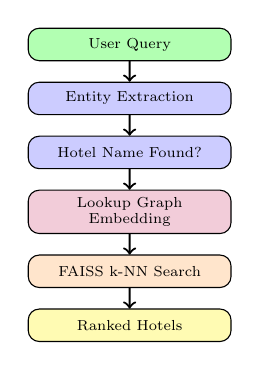
\begin{tikzpicture}[node distance=0.35cm, scale=0.75, transform shape,
    ebox/.style={rectangle, draw, fill=blue!20, text width=3.2cm, text centered, minimum height=0.55cm, rounded corners, font=\scriptsize}]

    \node[ebox, fill=green!30] (q1) {User Query};
    \node[ebox, below=of q1] (q2) {Entity Extraction};
    \node[ebox, below=of q2] (q3) {Hotel Name Found?};
    \node[ebox, below=of q3, fill=purple!20] (q4) {Lookup Graph Embedding};
    \node[ebox, below=of q4, fill=orange!20] (q5) {FAISS k-NN Search};
    \node[ebox, below=of q5, fill=yellow!30] (q6) {Ranked Hotels};

    \draw[->, thick] (q1) -- (q2);
    \draw[->, thick] (q2) -- (q3);
    \draw[->, thick] (q3) -- (q4);
    \draw[->, thick] (q4) -- (q5);
    \draw[->, thick] (q5) -- (q6);
\end{tikzpicture}
\end{center}

\end{column}

\begin{column}{0.5\textwidth}
\textbf{Key Insight:}
\begin{itemize}
    \scriptsize
    \item Graph embeddings encode structure, not text
    \item Query $\rightarrow$ Hotel $\rightarrow$ Embedding $\rightarrow$ FAISS
    \item Pre-computed embeddings stored in Neo4j
    \item Cosine similarity via FAISS IndexFlatIP
\end{itemize}

\vspace{0.2cm}
\textbf{Embedding Models:}
\begin{itemize}
    \scriptsize
    \item Node2Vec (128-dim) - Random walks
    \item FastRP (128-dim) - Random projection
\end{itemize}

\vspace{0.2cm}
\textbf{Function:}

\scriptsize
\texttt{search\_by\_query(query\_text, top\_k=5)}
\end{column}
\end{columns}
\end{frame}

%==============================================================================
%  ERROR ANALYSIS & IMPROVEMENTS
%==============================================================================
\section{Error Analysis \& Improvements}

\begin{frame}[t]{Error Analysis \& Limitations}
\vspace{0.2cm}
\textbf{Intent Classification:}
\begin{itemize}
    \setlength{\itemsep}{0.2em}
    \item Multi-intent queries not supported (``Find hotels and compare them'')
    \item Limited training data (200 generated samples)
    \item Out-of-domain queries classified with false confidence
    \item No intent hierarchy or fallback mechanism
\end{itemize}

\vspace{0.4cm}
\textbf{Entity Extraction:}
\begin{itemize}
    \setlength{\itemsep}{0.2em}
    \item Hotel names with special characters missed (L'Étoile)
    \item Relies on predefined keyword lists (not adaptive)
    \item spaCy NER misses domain-specific entities
    \item No coreference resolution (``that hotel'')
\end{itemize}
\end{frame}

%==============================================================================
% SECTION 3: GRAPH RETRIEVAL - BASELINE
%==============================================================================
\section{Graph Retrieval - Baseline}

\begin{frame}{Baseline Retrieval Pipeline}
\begin{center}
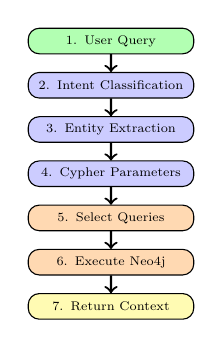
\begin{tikzpicture}[node distance=0.35cm, scale=0.65, transform shape,
    sbox/.style={rectangle, draw, fill=blue!20, text width=3cm, text centered, minimum height=0.5cm, rounded corners, font=\scriptsize}]

    \node[sbox, fill=green!30] (s1) {1. User Query};
    \node[sbox, below=of s1] (s2) {2. Intent Classification};
    \node[sbox, below=of s2] (s3) {3. Entity Extraction};
    \node[sbox, below=of s3] (s4) {4. Cypher Parameters};
    \node[sbox, below=of s4, fill=orange!30] (s5) {5. Select Queries};
    \node[sbox, below=of s5, fill=orange!30] (s6) {6. Execute Neo4j};
    \node[sbox, below=of s6, fill=yellow!30] (s7) {7. Return Context};

    \draw[->, thick] (s1) -- (s2);
    \draw[->, thick] (s2) -- (s3);
    \draw[->, thick] (s3) -- (s4);
    \draw[->, thick] (s4) -- (s5);
    \draw[->, thick] (s5) -- (s6);
    \draw[->, thick] (s6) -- (s7);

\end{tikzpicture}
\end{center}

\footnotesize
\textbf{Key Function:} \texttt{process\_query\_for\_baseline(user\_query, driver)}

\textbf{Flow:} Query $\rightarrow$ Intent $\rightarrow$ Entities $\rightarrow$ Params $\rightarrow$ Cypher $\rightarrow$ Neo4j $\rightarrow$ Context
\end{frame}



%------------------------------------------------------------------------------
\begin{frame}{Cypher Query Templates (1/2)}
\begin{columns}
\begin{column}{0.5\textwidth}
\textbf{Location Queries:}
\footnotesize

\vspace{0.1cm}
\texttt{-- Hotels in city}

\texttt{MATCH (h:Hotel)-[:LOCATED\_IN]->(c:City)}

\texttt{WHERE c.name = \$city}

\texttt{RETURN h.name, h.star\_rating}

\vspace{0.2cm}
\texttt{-- Top rated in country}

\texttt{MATCH (h:Hotel)-[:LOCATED\_IN]->(c:City)}

\texttt{~~~~~~-[:LOCATED\_IN]->(co:Country)}

\texttt{WHERE co.name = \$country}

\texttt{RETURN h.name ORDER BY h.star\_rating DESC}

\vspace{0.2cm}
\texttt{-- Cities with hotels}

\texttt{MATCH (h:Hotel)-[:LOCATED\_IN]->(c:City)}

\texttt{RETURN DISTINCT c.name, h.name}
\end{column}

\begin{column}{0.5\textwidth}
\textbf{Review Queries:}
\footnotesize

\vspace{0.1cm}
\texttt{-- Hotel reviews}

\texttt{MATCH (h:Hotel)<-[:REVIEWED]-(r:Review)}

\texttt{WHERE h.name = \$hotel\_name}

\texttt{RETURN r.text, r.score\_overall LIMIT 10}

\vspace{0.2cm}
\texttt{-- Reviews by demographic}

\texttt{MATCH (h:Hotel)<-[:REVIEWED]-(r:Review)}

\texttt{~~~~~~<-[:WROTE]-(t:Traveller)}

\texttt{WHERE h.name = \$hotel\_name}

\texttt{~~AND t.gender = \$gender}

\texttt{RETURN r.text, r.score\_overall}
\end{column}
\end{columns}
\end{frame}

%------------------------------------------------------------------------------
\begin{frame}{Cypher Query Templates (2/2)}
\begin{columns}
\begin{column}{0.5\textwidth}
\textbf{Visa \& Traveller Queries:}
\footnotesize

\vspace{0.1cm}
\texttt{-- Countries requiring visa}

\texttt{MATCH (tc:Country)-[:NEEDS\_VISA]->(co:Country)}

\texttt{WHERE tc.name = \$from\_country}

\texttt{RETURN co.name}

\vspace{0.2cm}
\texttt{-- Hotels without visa needed}

\texttt{MATCH (tc:Country), (h:Hotel)-[:LOCATED\_IN]}

\texttt{~~~~~~->(c:City)-[:LOCATED\_IN]->(co:Country)}

\texttt{WHERE tc.name = \$from AND NOT}

\texttt{~~~~~~(tc)-[:NEEDS\_VISA]->(co)}

\texttt{RETURN DISTINCT h.name}

\vspace{0.2cm}
\texttt{-- Best for traveller type}

\texttt{MATCH (h:Hotel)<-[:REVIEWED]-(r:Review)}

\texttt{~~~~~~<-[:WROTE]-(t:Traveller)}

\texttt{WHERE t.type = \$type}

\texttt{RETURN h.name, AVG(r.score\_overall)}
\end{column}

\begin{column}{0.5\textwidth}
\textbf{Rating \& Comparison:}
\footnotesize

\vspace{0.1cm}
\texttt{-- Hotels by cleanliness}

\texttt{MATCH (h:Hotel)}

\texttt{WHERE h.cleanliness\_base >= \$min}

\texttt{RETURN h.name, h.cleanliness\_base}

\texttt{ORDER BY h.cleanliness\_base DESC}

\vspace{0.2cm}
\texttt{-- Compare two hotels}

\texttt{MATCH (h1:Hotel), (h2:Hotel)}

\texttt{WHERE h1.name = \$hotel1}

\texttt{~~AND h2.name = \$hotel2}

\texttt{RETURN h1, h2}

\vspace{0.2cm}
\texttt{-- Hotels with most reviews}

\texttt{MATCH (h:Hotel)<-[:REVIEWED]-(r:Review)}

\texttt{RETURN h.name, COUNT(r) as cnt}

\texttt{ORDER BY cnt DESC LIMIT \$top\_n}

\vspace{0.3cm}
\textbf{Total: 31 Cypher Templates}
\end{column}
\end{columns}
\end{frame}

%------------------------------------------------------------------------------
\begin{frame}{Retrieved Data Examples}
\textbf{Query:} ``Recommend me a hotel in Tokyo''

\begin{columns}
\begin{column}{0.5\textwidth}
\textbf{Pipeline Output:}
\begin{itemize}
    \item Intent: hotel\_recommendation
    \item Entities: cities=[``Tokyo''], countries=[``Japan'']
\end{itemize}

\vspace{0.2cm}
\textbf{Cypher Results:}

\footnotesize
\begin{tabular}{|l|c|l|}
\hline
\textbf{Hotel} & \textbf{Rating} & \textbf{City} \\
\hline
The Azure Tower & 4.8 & Tokyo \\
Sakura Grand Hotel & 4.6 & Tokyo \\
Imperial Garden Inn & 4.5 & Tokyo \\
\hline
\end{tabular}
\end{column}

\begin{column}{0.5\textwidth}
\textbf{Query:} ``Best for business travelers''

\vspace{0.2cm}
\textbf{Pipeline Output:}
\begin{itemize}
    \item Intent: traveller\_preference
    \item Entities: traveller\_types=[``Business'']
\end{itemize}

\vspace{0.2cm}
\textbf{Cypher Results:}

\footnotesize
\begin{tabular}{|l|c|}
\hline
\textbf{Hotel} & \textbf{Avg Score} \\
\hline
Executive Suites & 9.2 \\
Business Bay Hotel & 8.9 \\
Corporate Tower & 8.7 \\
\hline
\end{tabular}
\end{column}
\end{columns}
\end{frame}

%==============================================================================
% SECTION 4: EMBEDDING-BASED RETRIEVAL
%==============================================================================

\section{Embedding-Based Retrieval}

\begin{frame}{Dual Node Embedding Approach}
\begin{center}
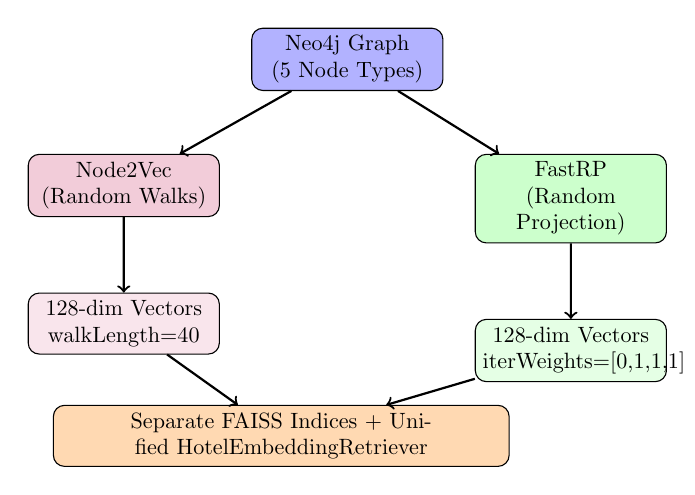
\begin{tikzpicture}[node distance=1.2cm, scale=0.8, transform shape,
    block/.style={rectangle, draw, fill=blue!20, text width=2.8cm, text centered, minimum height=0.9cm, rounded corners}]

    % Shared graph input
    \node[block, fill=blue!30] (graph) {Neo4j Graph\\(5 Node Types)};

    % Left side - Node2Vec
    \node[block, below left=1cm and 0.5cm of graph, fill=purple!20] (n2v) {Node2Vec\\(Random Walks)};
    \node[block, below=of n2v, fill=purple!10] (n2vemb) {128-dim Vectors\\walkLength=40};

    % Right side - FastRP
    \node[block, below right=1cm and 0.5cm of graph, fill=green!20] (frp) {FastRP\\(Random Projection)};
    \node[block, below=of frp, fill=green!10] (frpemb) {128-dim Vectors\\iterWeights=[0,1,1,1]};

    % FAISS
    \node[block, below=0.8cm of n2vemb, fill=orange!30, text width=7cm, xshift=2.5cm] (faiss) {Separate FAISS Indices + Unified HotelEmbeddingRetriever};

    % Arrows
    \draw[->, thick] (graph) -- (n2v);
    \draw[->, thick] (graph) -- (frp);
    \draw[->, thick] (n2v) -- (n2vemb);
    \draw[->, thick] (frp) -- (frpemb);
    \draw[->, thick] (n2vemb) -- (faiss);
    \draw[->, thick] (frpemb) -- (faiss);

\end{tikzpicture}
\end{center}

\end{frame}

%------------------------------------------------------------------------------
\begin{frame}{Embedding Models Comparison}
\begin{table}
\centering
\scriptsize
\begin{tabular}{lcc}
\toprule
\textbf{Property} & \textbf{Node2Vec} & \textbf{FastRP} \\
\midrule
Algorithm & Random Walks & Random Projection \\
Dimension & 128 & 128 \\
GDS Function & gds.node2vec.write() & gds.fastRP.write() \\
\midrule
Walk Length & 40 & -- \\
Iterations & 10 & -- \\
Iter. Weights & -- & [0.0, 1.0, 1.0, 1.0] \\
Computation Time & $\sim$2-3s & $\sim$0.2s \\
\midrule
Storage & Neo4j + FAISS & Neo4j + FAISS \\
Similarity & Cosine (via FAISS) & Cosine (via FAISS) \\
\bottomrule
\end{tabular}
\end{table}

\vspace{0.1cm}
\begin{columns}
\begin{column}{0.5\textwidth}
\textbf{Node2Vec Strengths:}
\begin{itemize}
    \scriptsize
    \setlength{\itemsep}{0.05em}
    \item Captures higher-order patterns
    \item Better structural similarity
    \item Flexible p,q parameters
    \item More expressive
\end{itemize}
\end{column}
\begin{column}{0.5\textwidth}
\textbf{FastRP Strengths:}
\begin{itemize}
    \scriptsize
    \setlength{\itemsep}{0.05em}
    \item 10x faster ($\sim$0.2s vs $\sim$2s)
    \item Memory efficient
    \item Good for large graphs
    \item Simpler hyperparameters
\end{itemize}
\end{column}
\end{columns}
\end{frame}

%------------------------------------------------------------------------------
\begin{frame}{Embedding Retrieval Results - Similar Hotels}
\begin{columns}
\begin{column}{0.5\textwidth}
\textbf{Node2Vec Search:}

Query Hotel: ``Berlin Mitte Elite''

\vspace{0.2cm}
\footnotesize
\begin{tabular}{|l|c|}
\hline
\textbf{Similar Hotel} & \textbf{Score} \\
\hline
Colosseum Gardens (Rome) & 0.686 \\
Aztec Heights (Mexico City) & 0.663 \\
Table Mountain View (Cape Town) & 0.587 \\
\hline
\end{tabular}

\vspace{0.2cm}
\textbf{Method:} Random walks capture neighborhood structure and traveller patterns
\end{column}

\begin{column}{0.5\textwidth}
\textbf{FastRP Search:}

Query Hotel: ``Berlin Mitte Elite''

\vspace{0.2cm}
\footnotesize
\begin{tabular}{|l|c|}
\hline
\textbf{Similar Hotel} & \textbf{Score} \\
\hline
The Kiwi Grand (Wellington) & 0.712 \\
Han River Oasis (Seoul) & 0.698 \\
Kremlin Suites (Moscow) & 0.685 \\
\hline
\end{tabular}

\vspace{0.2cm}
\textbf{Method:} Random projections capture immediate neighborhood relationships
\end{column}
\end{columns}

\vspace{0.3cm}
\textbf{Key Insight:} Both capture graph structure, but Node2Vec explores deeper paths while FastRP focuses on immediate neighbors.
\end{frame}

%------------------------------------------------------------------------------
\begin{frame}{Embedding Comparison in UI}
\begin{columns}
\begin{column}{0.5\textwidth}
\textbf{Side-by-Side Comparison:}

\vspace{0.2cm}
The UI displays results from both embedding models simultaneously when a hotel is mentioned or found in context.

\vspace{0.3cm}
\textbf{Example Query:} ``Tell me about The Azure Tower''

\vspace{0.2cm}
\footnotesize
\begin{tabular}{|l|c|}
\hline
\multicolumn{2}{|c|}{\textbf{Node2Vec Results}} \\
\hline
Colosseum Gardens & 0.739 \\
Tango Suites & 0.710 \\
The Royal Compass & 0.693 \\
\hline
\end{tabular}

\vspace{0.2cm}
\begin{tabular}{|l|c|}
\hline
\multicolumn{2}{|c|}{\textbf{FastRP Results}} \\
\hline
Gaudi's Retreat & 0.583 \\
Marina Bay Zenith & 0.567 \\
The Golden Oasis & 0.553 \\
\hline
\end{tabular}
\end{column}

\begin{column}{0.5\textwidth}
\textbf{Why Different Results?}

\vspace{0.2cm}
\begin{itemize}
    \scriptsize
    \item \textbf{Node2Vec:} Explores deeper graph paths via random walks
    \item \textbf{FastRP:} Captures immediate neighborhood via projections
    \item Same hotel can have different ``similar'' hotels
    \item Validates both models work independently
\end{itemize}

\vspace{0.3cm}
\textbf{UI Features:}
\begin{itemize}
    \scriptsize
    \item Automatic hotel extraction from query
    \item Falls back to first hotel in KG context
    \item Shows rank and similarity score
    \item Helps evaluate embedding quality
\end{itemize}

\vspace{0.2cm}
\textbf{Selected Model:} Sidebar dropdown chooses which embedding feeds into LLM context
\end{column}
\end{columns}
\end{frame}

%------------------------------------------------------------------------------
\begin{frame}{Error Analysis \& Improvement (Embeddings)}
\begin{columns}[T]
\begin{column}{0.5\textwidth}
\textbf{Error Analysis:}
\begin{itemize}
    \setlength{\itemsep}{0.3em}
    \item Graph embeddings are \textbf{not text encoders}
    \item Cannot convert text queries to vectors
    \item Requires hotel name extraction first
    \item Search fails if no hotel found
\end{itemize}
\end{column}

\begin{column}{0.5\textwidth}
\textbf{Improvement Added:}
\begin{itemize}
    \setlength{\itemsep}{0.3em}
    \item Fallback when no hotel name:
    \begin{itemize}
        \item Keyword match on city/country
        \item Use first hotel from KG context
    \end{itemize}
\end{itemize}
\end{column}
\end{columns}

\vspace{0.5cm}
\textbf{Key Limitations:}
\begin{enumerate}
    \small
    \setlength{\itemsep}{0.2em}
    \item Node embeddings + FAISS don't use Cypher $\rightarrow$ relationships only captured implicitly via node walks. Both \textbf{relationships} and \textbf{directionality} are lost.
    \item Vector similarity finds fuzzy matches — for precise queries (numbers, names), we must apply custom filters first, then run hybrid retrieval.
\end{enumerate}
\end{frame}

%==============================================================================
% SECTION 5: LLM LAYER
%==============================================================================
\section{LLM Layer}

\begin{frame}{LLM Context Construction}
\large
\textbf{Process Flow:}

\vspace{0.5cm}
\begin{enumerate}
    \setlength{\itemsep}{0.4cm}
    \item \textbf{Intent Classification}
    \begin{itemize}
        \item Classify the intent of user query to select relevant Cypher templates
    \end{itemize}

    \item \textbf{Entity Extraction}
    \begin{itemize}
        \item Extract entities from user query to fill in Cypher template parameters
    \end{itemize}

    \item \textbf{Graph Retrieval}
    \begin{itemize}
        \item Execute selected Cypher queries on Neo4j database
    \end{itemize}

    \item \textbf{Context Merge}
    \begin{itemize}
        \item Combine all results to build the final context for LLM
    \end{itemize}
\end{enumerate}

\end{frame}

%------------------------------------------------------------------------------
\begin{frame}{Intent-to-Query Mapping}
\footnotesize
\begin{tabular}{|l|p{8cm}|}
\hline
\textbf{Intent} & \textbf{Cypher Queries Selected} \\
\hline
hotel\_recommendation & get\_top\_rated\_hotels\_in\_city, get\_top\_rated\_hotels\_in\_country \\
\hline
hotel\_search & get\_hotels\_by\_rating, get\_hotels\_in\_city\_by\_rating, get\_hotels\_in\_country\_by\_rating \\
\hline
hotel\_info & get\_hotel\_info \\
\hline
review\_query & get\_hotel\_reviews, get\_hotel\_review\_count, get\_latest\_hotel\_reviews, get\_hotel\_reviews\_filtered \\
\hline
comparison & compare\_two\_hotels \\
\hline
traveller\_preference & get\_best\_hotels\_for\_traveller\_type, get\_best\_hotels\_for\_gender, get\_best\_hotels\_for\_age\_group \\
\hline
location\_query & get\_hotels\_in\_city, get\_hotels\_in\_country, get\_cities\_in\_country \\
\hline
visa\_query & get\_countries\_requiring\_visa, get\_hotels\_accessible\_without\_visa \\
\hline
rating\_filter & get\_hotels\_by\_cleanliness\_base, get\_hotels\_by\_comfort\_base, get\_hotels\_by\_facilities\_base \\
\hline
general\_question & get\_all\_hotels \\
\hline
\end{tabular}

\vspace{0.3cm}
\normalsize
\textbf{Total:} 31 Cypher query templates mapped to 10 intents
\end{frame}

%------------------------------------------------------------------------------
\begin{frame}{Prompt Structure}
\textbf{Persona Definition:}

\footnotesize
``You are J.A.R.V.I.S., an advanced AI hotel concierge assistant.
You speak with sophisticated eloquence and always address the user as 'sir' or 'madam'.
Your responses are warm yet professional, helpful and conversational - never robotic or formulaic.
NEVER start responses with phrases like 'Based on the data provided' or 'According to the information'.
Instead, speak naturally as if you personally know these hotels and are offering genuine recommendations.''

\vspace{0.3cm}
\normalsize
\textbf{Key Instructions:}

\footnotesize
\begin{itemize}
    \item Address the user respectfully as ``sir'' at least once
    \item Be conversational and natural, as if having a pleasant discussion
    \item Provide specific details from the data without mentioning "the data" or "the context"
    \item Use the Hotel information data available below (that was retrieved based on the query) as context/baseline information to help with the recommendations.
    \item If recommending hotels display ranked recommendations with explanations. Show why certain entities were recommended based on user preferences and KG data 
    \item Keep responses concise but informative
\end{itemize}
\end{frame}

%------------------------------------------------------------------------------
\begin{frame}{Context Injection}
\begin{columns}[T]
\begin{column}{0.5\textwidth}
\textbf{Baseline Context Injection:}
\begin{itemize}
    \item Hotel information from KG retrieval (Cypher queries) is appended to the prompt
\end{itemize}
\end{column}

\begin{column}{0.5\textwidth}
\textbf{Embeddings Context:}
\begin{itemize}
    \item LLM is given a retriever that performs similarity search on embeddings
    \item Finds hotels similar to the one mentioned in query
\end{itemize}
\end{column}
\end{columns}

\vspace{0.4cm}
\textbf{Combined Approach:} Both baseline (explicit KG data) and embedding (implicit similarity) contexts are merged to provide comprehensive information to the LLM.
\end{frame}

%------------------------------------------------------------------------------
\begin{frame}{LLM Comparison - Quantitative Results}
\begin{table}
\centering
\begin{tabular}{lccccc}
\toprule
\textbf{Model} & \textbf{Latency (s)} & \textbf{Input Tok} & \textbf{Output Tok} & \textbf{Cost (\$)} & \textbf{Sem. Acc.} \\
\midrule
Gemma-2-2B & 0.51 & 6 & 31 & 0.000007 & 0.057 \\
Mistral-7B & 10.60 & 6 & 211 & 0.000128 & 0.037 \\
LLaMA-3.1-8B & 4.63 & 6 & 382 & 0.000307 & 0.252 \\
\bottomrule
\end{tabular}
\caption{Performance Metrics (averaged across test queries)}
\end{table}

\vspace{0.1cm}
\footnotesize
\textbf{Semantic Accuracy Calculation:}
\begin{itemize}
    \setlength{\itemsep}{0.05em}
    \item \textbf{Method:} Cosine similarity (SentenceTransformer) between LLM response and reference embeddings
    \item \textbf{Test Query:} ``Hotels recommended for seniors''
    \item \textbf{Reference:} ``Canal House Grand in Amsterdam, high comfort/cleanliness score, fantastic location.''
\end{itemize}

\vspace{0.1cm}
\textbf{Cost:} HuggingFace API pricing/1K tokens \quad \textbf{Integration:} LangChain + HuggingFace Inference API
\end{frame}

%------------------------------------------------------------------------------
\begin{frame}{LLM Comparison - Qualitative Evaluation}
\begin{columns}
\begin{column}{0.33\textwidth}
\textbf{Gemma-2-2B}
\begin{itemize}
    \scriptsize
    \item Fastest response
    \item Concise answers
    \item Sometimes incomplete
    \item Good for simple queries
\end{itemize}
\end{column}

\begin{column}{0.33\textwidth}
\textbf{Mistral-7B}
\begin{itemize}
    \scriptsize
    \item Balanced performance
    \item Good reasoning
    \item Handles complex queries
    \item Best cost/quality ratio
\end{itemize}
\end{column}

\begin{column}{0.33\textwidth}
\textbf{LLaMA-3.1-8B}
\begin{itemize}
    \scriptsize
    \item Most detailed
    \item Best accuracy
    \item Higher latency
    \item Best for complex tasks
\end{itemize}
\end{column}
\end{columns}

\vspace{0.5cm}
\begin{center}
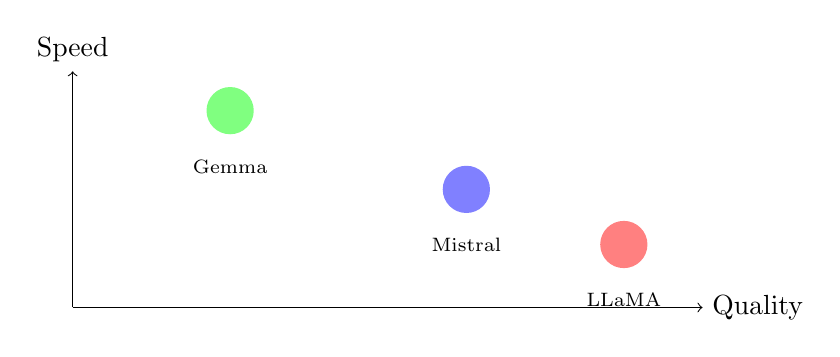
\begin{tikzpicture}
    \draw[->] (0,0) -- (8,0) node[right] {Quality};
    \draw[->] (0,0) -- (0,3) node[above] {Speed};

    \node[circle, fill=green!50, minimum size=0.6cm] at (2,2.5) {};
    \node[below] at (2,2) {\scriptsize Gemma};

    \node[circle, fill=blue!50, minimum size=0.6cm] at (5,1.5) {};
    \node[below] at (5,1) {\scriptsize Mistral};

    \node[circle, fill=red!50, minimum size=0.6cm] at (7,0.8) {};
    \node[below] at (7,0.3) {\scriptsize LLaMA};
\end{tikzpicture}
\end{center}
\end{frame}
%------------------------------------------------------------------------------
\begin{frame}{Error Analysis \& Improvement (LLM)}
\begin{columns}[T]
\begin{column}{0.5\textwidth}
\textbf{Errors Encountered \& Fixed:}
\begin{itemize}
    \setlength{\itemsep}{0.2em}
    \item \textbf{Robotic responses:} LLM started with Basic robotic phrases
    \begin{itemize}
        \item Fixed via persona prompt engineering
    \end{itemize}
\end{itemize}
\end{column}

\begin{column}{0.5\textwidth}
\textbf{Remaining Limitations:}
\begin{itemize}
    \setlength{\itemsep}{0.2em}
    \item \textbf{Gemma-2-2B:} Often gives incomplete answers due to small model size
    \item \textbf{Low semantic accuracy:} Models struggle to match reference answers exactly
    \item \textbf{Context length:} Large KG results may exceed token limits
    \item \textbf{No memory:} Each query is independent, no conversation history
\end{itemize}
\end{column}
\end{columns}
\end{frame}

%==============================================================================
% SECTION 7: LIVE DEMO
%==============================================================================
\section{Live Demo}

\begin{frame}{Pipeline Recap for Demo}
\begin{center}
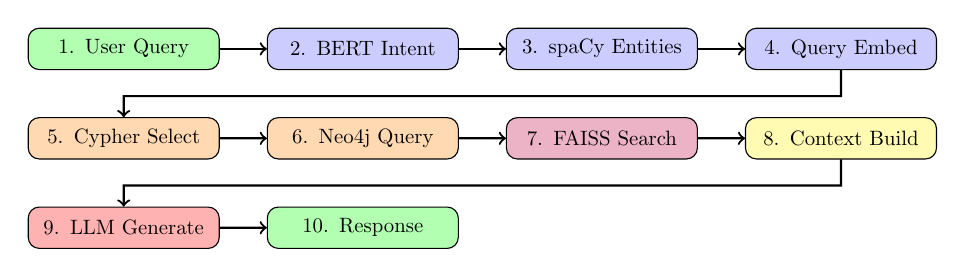
\begin{tikzpicture}[node distance=0.8cm, scale=0.75, transform shape,
    pstep/.style={rectangle, draw, fill=blue!20, text width=3cm, text centered, minimum height=0.7cm, rounded corners}]

    \node[pstep, fill=green!30] (s1) {1. User Query};
    \node[pstep, right=of s1] (s2) {2. BERT Intent};
    \node[pstep, right=of s2] (s3) {3. spaCy Entities};
    \node[pstep, right=of s3] (s4) {4. Query Embed};

    \node[pstep, below=0.8cm of s1, fill=orange!30] (s5) {5. Cypher Select};
    \node[pstep, right=of s5, fill=orange!30] (s6) {6. Neo4j Query};
    \node[pstep, right=of s6, fill=purple!30] (s7) {7. FAISS Search};
    \node[pstep, right=of s7, fill=yellow!30] (s8) {8. Context Build};

    \node[pstep, below=0.8cm of s5, fill=red!30] (s9) {9. LLM Generate};
    \node[pstep, right=of s9, fill=green!30] (s10) {10. Response};

    \draw[->, thick] (s1) -- (s2);
    \draw[->, thick] (s2) -- (s3);
    \draw[->, thick] (s3) -- (s4);
    \draw[->, thick] (s4) -- ++(0,-0.8) -| (s5);
    \draw[->, thick] (s5) -- (s6);
    \draw[->, thick] (s6) -- (s7);
    \draw[->, thick] (s7) -- (s8);
    \draw[->, thick] (s8) -- ++(0,-0.8) -| (s9);
    \draw[->, thick] (s9) -- (s10);

\end{tikzpicture}
\end{center}

\vspace{0.3cm}
\textbf{Demo Features:}
\begin{itemize}
    \item Switch between embedding models (Node2Vec / FastRP)
    \item Switch between LLMs (Gemma / Mistral / LLaMA)
    \item Side-by-side embedding comparison
    \item Streamlit UI with J.A.R.V.I.S. persona
\end{itemize}
\end{frame}

%------------------------------------------------------------------------------
\begin{frame}{Demo Queries}
\textbf{Test Queries for Live Demo (Pre-loaded in UI):}

\begin{enumerate}
    \item \textbf{Recommendation:} ``Recommend me a good hotel in Tokyo''

    \item \textbf{Search:} ``Find hotels in Paris''

    \item \textbf{Hotel Info:} ``Tell me about The Azure Tower''

    \item \textbf{Reviews:} ``Show me reviews for The Golden Oasis''

    \item \textbf{Comparison:} ``Compare The Azure Tower and L'Etoile Palace''

    \item \textbf{Traveller:} ``Best hotels for business travelers''

    \item \textbf{Rating Filter:} ``Hotels with cleanliness rating above 9''

    \item \textbf{Demographics:} ``Hotels recommended for seniors''
\end{enumerate}

\vspace{0.3cm}
\begin{center}
\textbf{[LIVE DEMO]}
\end{center}
\end{frame}

%==============================================================================
\begin{frame}
\begin{center}
\Huge Thank You!

\vspace{1cm}
\Large Questions?
\end{center}
\end{frame}

\end{document}
